% =====================================================================
% Hashim Almodamagha -- RIT ALGO1 write-up (HW3, section "RIT Simulation 2")
%
% Where it goes: save as sections/rit_hashim.tex and add
%     \input{sections/rit_hashim}
% in sections/rit_team.tex just above \appendix (after Alexander's section).
% The appendix listing is in rit_hashim_appendix.tex: save it as
% sections/rit_hashim_appendix.tex and \input it at the very end of
% rit_team.tex (after Alexander's script).
%
% Files to upload to Overleaf:
%   figures/ha_algo1_session.pdf   (built from my run logs)
%   figures/ha_rit_pnl.png         (P&L chart cropped from my RIT screenshot)
%   sections/algo1_arbitrage.py    (my script, unchanged; the appendix quotes
%                                   line ranges from it)
%
% Uses only packages main.tex already loads (graphicx, float, booktabs,
% listings, xcolor). The price path is not repeated here: the text points to
% Giancarlo's Figure \ref{fig:ga_final}, which shows the same graded case.
%
% Before submitting, fill the two \todoTM placeholders (what ran between
% ticks 77 and 157). Search for "todoTM".
%
% Sources for the numbers: the logs of my three runs on 2026-09-10 (practice
% 19:22, graded 20:04 and 20:14), the RIT screenshot at the close, and the
% run-3 .log (17 attempts / 7 one-legged / ~$500 of unwinds; that file is not
% in the PS3 folder, the figures come from ALGO1_brief.md).
% =====================================================================

\subsection{Hashim Almodamagha}

\paragraph{a. Strategy going in.}
CRZY trades on two exchanges, \texttt{CRZY\_M} and \texttt{CRZY\_A}, with separate
books but one combined position, so a share bought on one and sold on the other
leaves me flat. The trade the case is built around is the crossed market: when the
bid on one exchange is above the ask on the other, buy on the cheap side, sell on the
rich side and keep the difference. I expected every script in the room to be
watching the same crosses, so I did not want my whole result to depend on winning
that race. My script ran two strategies in the same loop, the crossed-market
arbitrage and a market maker that kept a bid and an ask on both exchanges to earn the
spread from everyone else's order flow. Every parameter lived in an Excel sheet that
the script re-read four times a second, so I could change sizes and spreads during
the case without restarting it.

\textbf{Arbitrage.} Each loop pulled twenty levels of both books, with my own orders
removed so the bot could never mistake its own quotes for a cross. When a cross
cleared a one-cent minimum edge, net of a per-share cost on each leg (zero in this
case, but it is the input discussion question 1 asks for), the script sent a
marketable limit buy at the ask it had seen and a marketable limit sell at the bid it
had seen, then cancelled whatever had not filled. Pricing at the observed quote meant
that if the cross had already gone, the order would not fill rather than fill at a
bad price. If only one leg filled, the leftover was closed straight away, first with
a limit order at the best price across both exchanges and then with a market order
for anything still open, and the arbitrage paused for two seconds.

\textbf{Market making.} With $m$ the consolidated mid (best bid and best ask across
both exchanges) and $q$ my net position, the quotes were
\begin{equation*}
h=\max\bigl(h_0,\ \text{range of } m \text{ over the last 3 s},\ s_{\min}/2\bigr),\qquad
\text{bid}=m-h-\gamma q,\qquad \text{ask}=m+h-\gamma q,
\end{equation*}
with a base half spread $h_0$ of 3 to 4 cents (I moved it between the two during the
session), an optional floor $s_{\min}$ I could set by hand, and an inventory skew
$\gamma$ of 3 cents per 1{,}000 shares, so a long position pushed both quotes down
and a short one pushed them up. Quotes were clamped so they never crossed the other
exchange, and beyond an inventory cap the side that would add to the position was
pulled.

\textbf{Risk controls.} A self-imposed 15{,}000-share gross cap, below the case's
25{,}000; after the practice run, a ``hard flat'' that cancelled the quotes and
market-flattened the position if $|q|$ reached 5{,}000 shares; Flatten and Panic
switches in the sheet; and a throttle at 80 API calls per second.

\paragraph{b. What happened and size strategy.}

\textbf{Size strategy.} For the arbitrage the script walked the cheap exchange's asks
against the rich exchange's bids level by level, the way a matching engine would,
adding shares only while every share still cleared the minimum edge. That gives the
quantity that is actually crossable rather than whatever size is displayed at the
top. The result was capped at 2{,}000 shares, at the 10{,}000-share order limit and
at the room left under my 15{,}000 cap after counting my resting quotes. I chose the
2{,}000 cap because a cross was usually one small order priced through a deep level,
so there was rarely more than a few thousand shares to take, and a one-legged fill
of 2{,}000 shares was a leftover I could close for a few dollars. This is the
trade-off in discussion question 4: without the order limit the walk would size
larger and earn more per cross, but the position left behind by a missed leg grows
one for one with the size. For market making the size was a fixed number of shares
per quote, cut to whatever room was left. I changed it several times during the
session, between 600 and 2{,}000 shares.

\textbf{Practice run.} The first version of the script ran a full practice case and
exposed three things about the RIT server that I had not designed for.
\begin{enumerate}
  \item The response to \texttt{POST /orders} is the order \emph{before} it is
        matched, so it shows nothing filled even when the order filled at once, and
        \texttt{GET /orders/\{id\}} returns 404 once an order has filled. The
        re-read of my own orders returned 404 in all 26 arbitrage attempts, so
        every ``one-legged'' result was a guess. At tick 21, where the log lets me
        check, both legs of a 2{,}000-share arbitrage had filled. The bot concluded
        the sell had not and ``closed'' a leftover that did not exist with a
        2{,}000-share market sell, which turned a 3-cent arbitrage into a
        2{,}000-share short. Only one of the 26 attempts was recorded as complete
        (+\$60).
  \item New orders appear in the list of open orders 0.1 to 0.6 seconds late. The
        market maker took a missing quote to mean a filled one, lost track of 401
        of its own quotes, re-posted duplicates, and the forgotten quotes filled
        later without the bot seeing them. Of the 29 orders still open at the end,
        23 were such quotes.
  \item RIT reports the combined CRZY position on \emph{both} tickers, so adding
        the two, which is what my code did, doubled it.
\end{enumerate}
The run made \$3{,}498, but from the direction of the price, not from the strategy.
Before the graded case I patched the first two: every order is now looked up in the
open, filled and cancelled lists, with a grace period before it counts as gone, and
any open order that nothing in the script is tracking gets cancelled. I also added
the hard flat. I did not catch the third.

\textbf{The graded case.} Figure~\ref{fig:ha_session} shows the case from my logs,
and Giancarlo's Figure~\ref{fig:ga_final} shows the price path, from \$10.00 up to
about \$13.10 by tick 170 and back to \$9.94 at the close.

\begin{figure}[ht]
  \centering
  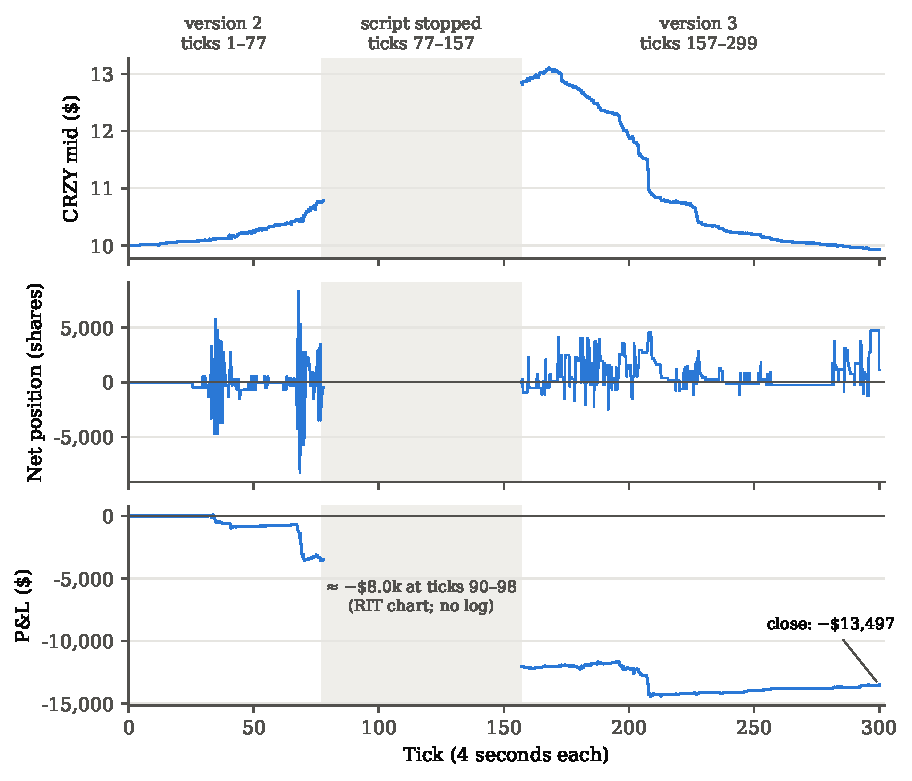
\includegraphics[width=0.9\linewidth]{figures/ha_algo1_session.pdf}
  \caption{My graded case, from the script's logs. Top: consolidated mid of CRZY.
  Middle: my true net position (the first-patch version logged twice the real
  figure; it is halved here). The spikes at ticks 33--40 and 67--76 are the 18
  forced flattens, each of which flipped the sign of the position. Bottom: P\&L,
  from RIT's realized and unrealized figures. No script of mine logged anything
  between ticks 77 and 157 (shaded); Figure~\ref{fig:ha_rit} covers that stretch.}
  \label{fig:ha_session}
\end{figure}

\emph{Ticks 1--77, first patch.} The patch did its job: the lost quotes were gone.
The double count was still there, and the arbitrage leftover was now worked out from
the change in position, which was doubled and also picked up market-making fills
from the same instant. Twice the bot ``closed'' 8{,}000 shares when its orders said
2{,}000 had filled. That pushed the position past the hard flat, and the hard flat
read the same doubled position: it market-sold twice the real position, which
flipped it to the other side, saw the flipped position (doubled again) two seconds
later and flipped it back. This happened 18 times, each one a market order of 4{,}500
to 10{,}600 shares paying the spread. The arbitrage completed none of its 7 attempts.
The market maker on its own was slightly positive, +\$319 marked against the mid
three seconds after each fill. I stopped the script at tick 77 at $-\$3{,}555$.

\emph{Ticks 77--157.} I have no log for this stretch. RIT's own P\&L chart
(Figure~\ref{fig:ha_rit}) shows the account dropping about \$8{,}500 in a few
seconds around ticks 93--97, \todoTM{what was running then: e.g.\ ``when I
restarted the first-patch version, which ...'' or ``when I traded by hand ...''}.

\begin{figure}[ht]
  \centering
  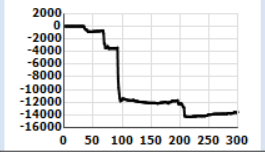
\includegraphics[width=0.45\linewidth]{figures/ha_rit_pnl.png}
  \caption{P\&L of my account by tick, from the RIT client at the close. It is the
  only record of ticks 77--157, where it shows the drop of about \$8{,}500 around
  ticks 93--97.}
  \label{fig:ha_rit}
\end{figure}

\emph{Ticks 157--300, second patch.} The second patch read the position from one
ticker only and worked out an arbitrage leftover from the fills of its two legs
instead of the position change. The mechanics were clean, with no accounting
mismatches and no forced flattens, and the run lost \$1{,}431, from $-\$12{,}066$ to
$-\$13{,}497$.
\begin{itemize}
  \item \textbf{Arbitrage: none of 17 attempts completed, and 7 filled one leg.}
        Closing those leftovers cost about \$500. In the practice run, where the bot
        looked at the books every few milliseconds, a cross lasted about 0.2 seconds
        at the median. In the graded case the crossed quote was gone by the time my
        orders arrived, and my two legs went out one after the other. The leg that
        filled was always the one on the deep, normal side of the book, the one
        nobody else was racing for.
  \item \textbf{Market making earned the spread.} 268 fills and 264{,}638 shares, for
        +\$3{,}760 against the mid when each fill was recorded (1.4 cents a share)
        and +\$3{,}108 against the mid three seconds later (1.2 cents a share).
  \item \textbf{Inventory lost more than the spread made, about \$4{,}700.} Between
        ticks 195 and 215 the price fell from \$12.29 to \$10.78, and the bot was
        long for 94\% of that stretch, by 1{,}820 shares on average. The buyers who
        had been lifting my ask disappeared and sellers kept hitting my bid. A skew
        of 3 cents per 1{,}000 shares moved my quotes less than the price moved in a
        second, so the quotes kept buying a falling stock, and I had raised the quote
        size to 2{,}000 shares shortly before the drop.
  \item \textbf{The close.} The script had no end-of-case flatten. Once the
        simulation stopped, the server rejected its orders and I finished holding
        1{,}128 shares.
\end{itemize}

\paragraph{c. MARKET vs.\ LIMIT orders.}
A market order fixes the quantity and accepts whatever price it takes to fill it,
walking down the book until it is done: execution is certain, price is not. A limit
order fixes the worst price I will accept. It fills at that price or better, and the
rest either rests in the book or is cancelled: price is certain, execution is not.

\textbf{The risk of a market order is price, and it executes whatever the bot
believes.} The textbook risk is slippage. A cross in this case is one small order
priced through levels that are tens of thousands of shares deep, so a market order
bigger than the crossing order fills the rest at ordinary prices, and on a 1- to
3-cent edge one level of slippage erases the profit. That is why my arbitrage legs
were never market orders. The risk that actually cost me money was a different one.
A market order is immediate and cannot be taken back, so it carries out whatever the
bot believes, right or wrong. In the first-patch run every market order I sent was
an emergency order, a leftover close or a hard flat, and every one of them was sized
from a position reading that was twice the truth. Those orders are essentially the
whole of that run's loss.

\textbf{The risk of a limit order is execution, plus adverse selection while it
rests.} For a two-legged arbitrage, non-execution means legging risk: one leg fills,
the other does not, and I hold a position in a stock I had no view on. That was 7 of
17 attempts in the final run. A resting limit order has a second risk. It is a free
option for the rest of the market, and it gets exercised when the price moves
through it. My market maker was made of resting limit orders on purpose, and both
sides of that showed up in the data. The quotes earned about 1.4 cents a share at the
fill and kept about 1.2 cents three seconds later, so in normal trading the spread
more than paid for the adverse selection. In the drop the bids kept getting hit as
the price fell through them, and that is where the inventory loss came from. The
quotes the practice version had forgotten about were the same risk without any
monitoring at all: limit orders still resting in the book that filled later, unseen.

\textbf{What I used.} Marketable limits for both arbitrage legs, because a 1- to
3-cent edge cannot afford slippage. A limit and then a market order to close a
leftover, because being flat mattered more than the last cent. Market orders only for
emergency flattens. Resting limits only for market making, refreshed every second
(every 0.1 seconds by the end) to keep stale quotes from being picked off.

\paragraph{d. P\&L and lessons.}
My final P\&L was $\mathbf{-\$13{,}497.17}$, with no fines. Table~\ref{tab:ha_pnl}
splits it by stretch of the case.

\begin{table}[ht]
  \centering\small
  \begin{tabular}{llrp{0.42\linewidth}}
    \toprule
    Stretch & Ticks & P\&L (\$) & What drove it\\
    \midrule
    First patch    & 1--77    & $-3{,}555$  & double-counted position: inflated leftover
                                              closes and 18 forced flattens\\
    No logged run  & 77--157  & $-8{,}511$  & \todoTM{cause}\\
    Second patch   & 157--300 & $-1{,}431$  & spread $+3{,}760$, arbitrage leftovers
                                              about $-500$, inventory about $-4{,}700$\\
    \midrule
    Total          &          & $-13{,}497$ & \\
    \bottomrule
  \end{tabular}
  \caption{My P\&L in the graded case, by stretch. The endpoints are RIT's figures
  when I stopped the first-patch script, when the second-patch script started, and
  at the close.}
  \label{tab:ha_pnl}
\end{table}

Four lessons, in order of what they cost.
\begin{enumerate}
  \item \textbf{Know what the server aggregates.} RIT reports the combined CRZY
        position, and the realized P\&L, on each ticker. Adding the two doubled
        both, and the doubled position caused the whole first-patch loss. Giancarlo
        hit the same problem in practice.
  \item \textbf{A safety rule is only as good as the number it acts on.} The hard
        flat was meant to cap my losses, and fed a doubled position it became the
        largest logged source of them. A rule that sends market orders should
        confirm the position from two independent reads, or from the fills
        themselves, before it fires, and it should never fire twice on the same
        stale number.
  \item \textbf{Never trust a single response from the server.} The answer to an
        order is a snapshot from before the match, a lookup can 404 on an order that
        filled, and the open-order list lags. Every order has to be reconciled
        against all three lists, with a grace period.
  \item \textbf{The market-making edge was real, and inventory decided the result
        anyway.} About 1.2 cents a share survived adverse selection, but a few
        thousand shares of inventory through a fall of \$1.50 in twenty seconds
        cost more than the spread made all run. Next time I would scale the skew
        with how fast the price is moving, stop quoting the side a trend is
        running over, and flatten before the close.
\end{enumerate}
On the arbitrage itself (discussion question 3), at my speed it could not be won:
the crossed quote was gone before my orders landed, so I only ever got the leg
nobody else wanted. My teammates' results show the two ways around this. Charishma
sent both legs at once with very little latency, and Giancarlo sent the scarce leg
first and hedged only what filled. Both made money.

The same code also answers discussion question 5, and not well. If the Alternate
exchange halted with its last quotes still on screen, the bot would keep seeing a
cross. The Main leg would fill, the Alternate order would be rejected, and the
script would treat the filled leg as a leftover to close. The close goes to whichever
exchange shows the better price, though, and that could be the halted one, so the
close would fail and leave the position open. Two seconds later the pause would
expire and the bot would fire at the same stale cross again. The fix is to stop
routing to an exchange after a few rejections in a row, which is what Charishma
added.

\paragraph{The script and how to use it.} The script is
\texttt{algo1\_arbitrage.py}; the key functions are in the appendix and the full file
is submitted with the report. It needs Python 3 with \texttt{requests}, and
\texttt{xlwings} with Excel for the control sheet (without Excel it runs on the
defaults at the top of the file).
\begin{enumerate}
  \item In the RIT client, turn on the API from the status bar and note the port and
        API key. Put them in \texttt{API\_KEY} and \texttt{PORT} at the top of the
        script.
  \item Run it (F5 in Spyder, or \texttt{python algo1\_arbitrage.py}). It can start
        before the case: while the case is paused or stopped it waits, with no
        quotes out.
  \item It opens \texttt{ALGO1\_cockpit.xlsx}, creating it the first time. The yellow
        cells on the \emph{Control} sheet are the parameters and are read live.
        \emph{Live} shows both books, the crosses, my quotes, position and P\&L about
        five times a second, and \emph{Trades} lists every arbitrage and fill.
  \item Market making starts switched off: set \texttt{MM enabled} to 1 to quote.
        \texttt{Enabled} = 0 turns the whole bot into watch-only.
  \item \texttt{Flatten now} = 1 cancels the quotes and closes the position without
        stopping. \texttt{Panic} = 1, or Ctrl+C, cancels everything, flattens and
        stops the script. It never stops on its own.
  \item Each run writes a \texttt{.log}, a per-loop \texttt{\_ticks.csv}, a
        \texttt{\_trades.csv} and a final \texttt{\_orders.csv} to a \texttt{logs}
        folder next to the script. This write-up is built from them.
\end{enumerate}
